\documentclass[10pt]{article}
\usepackage{tikz}
\usepackage[margin=0cm]{geometry}
\pagestyle{empty}

\begin{document}

\vspace*{\fill}
\begin{center}
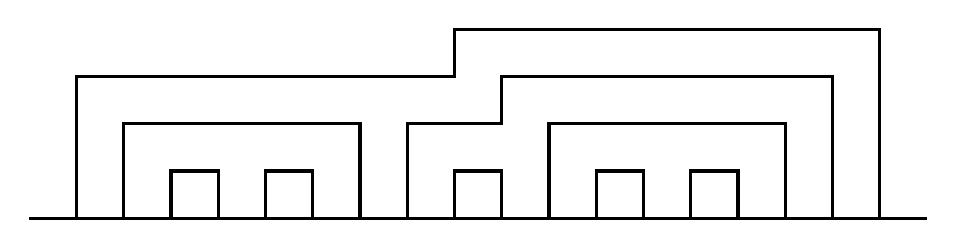
\begin{tikzpicture}[x=0.6cm, y=0.6cm, very thick]
\draw (-1,0) -- (18,0);
% Arch 1
    \draw (0,0) -- (0,3) -- (8,3) -- (8,4) -- (17,4) -- (17,0);
% Arch 2
    \draw (1,0) -- (1,2) -- (6,2) -- (6,0);
% Arch 3
    \draw (2,0) -- (2,1) -- (3,1) -- (3,0);
% Arch 4
    \draw (4,0) -- (4,1) -- (5,1) -- (5,0);
% Arch 5
    \draw (7,0) -- (7,2) -- (9,2) -- (9,3) -- (16,3) -- (16,0);
% Arch 6
    \draw (8,0) -- (8,1) -- (9,1) -- (9,0);
% Arch 7
    \draw (10,0) -- (10,2) -- (15,2) -- (15,0);
% Arch 8
    \draw (11,0) -- (11,1) -- (12,1) -- (12,0);
% Arch 9
    \draw (13,0) -- (13,1) -- (14,1) -- (14,0);
\end{tikzpicture}
\end{center}
\vspace*{\fill}

\end{document}
